%  Beamer slide example.

\documentclass[9pt]{beamer}
%\setbeameroption{show only notes}
%\setbeameroption{show notes}

\usepackage[utf8]{inputenc}
\usetheme{inria}
\usepackage{helvet}
\usepackage{graphicx}

\usepackage{tikz}
\usetikzlibrary{arrows,shapes,positioning,calc,shadows,trees}
\tikzset{
  mstep1/.style = {basic, rounded corners=2pt, thin, align=center, fill=orange!70,text width=1.5cm},
  mstep2/.style = {basic, rounded corners=2pt, thin, align=center, fill=green!30,text width=1.5cm},
  mstep2b/.style = {basic, rounded corners=2pt, thin, align=center, fill=white,text width=2cm},
  mstep3/.style = {basic, rounded corners=2pt, thin, align=center, fill=green!30,text width=3cm},
  mstep3b/.style = {basic, rounded corners=2pt, thin, align=center,fill=white,text width=7cm},
  mstep4/.style = {basic, thin, align=left, fill=gray!60, text width=6.5em},
  basic/.style  = {draw, text width=2cm, drop shadow, font=\sffamily, rectangle},
  root/.style   = {basic, rounded corners=2pt, thin, align=center,
  fill=green!30},
  level 2/.style = {basic, rounded corners=6pt, thin,align=center, fill=green!60,
  text width=8em},
  level 3/.style = {basic, thin, align=left, fill=orange!60, text width=6.5em},
  mlevel4/.style = {basic, thin, align=left, fill=gray!60, text width=6.5em}
}
\tikzstyle{every picture}+=[remember picture]
\tikzstyle{na} = [baseline=-.5ex]


\def\aboxl[#1,#2,#3,#4,#5]#6{%
  \node[draw, cylinder, alias=cyl, shape border rotate=90, aspect=#3, %
    minimum height=#1, minimum width=#2, outer sep=-0.5\pgflinewidth, %
    color=orange!40!black, left color=orange!70, right color=orange!80, middle
  color=white] (#4) at #5 {};%
  \node at #5 {#6};%
  \fill [orange!30] let \p1 = ($(cyl.before top)!0.5!(cyl.after top)$), \p2 =
  (cyl.top), \p3 = (cyl.before top), \n1={veclen(\x3-\x1,\y3-\y1)},
\n2={veclen(\x2-\x1,\y2-\y1)} in (\p1) ellipse (\n1 and \n2); }

\author{Soraya Arias \and Maurice Brémond \and Gaëtan Harter \and David Parsons}

\title[CI]{Continuous Integration at INRIA}
% \subtitle{Dans un contexte de développement Inria}
\subtitle{Practical seminar, xx xx 2015}

% Automatically insert a "new section" page at each section.
\AtBeginSection[]{
  \begin{frame}[plain]
    \partpage
  \end{frame}
}
% \inriaswitchcolors COLOR
%
% Where COLOR is one of red, blue, orange, darkblue, violet,
% pastelgreen, grey, or green.
\newcommand{\inriaswitchcolors}[1]{%
  \pgfaliasimage{figfootline}{figfootline-#1}% !!!
  \pgfaliasimage{figbackground}{figbackground-#1}% !!!
  \pgfaliasimage{figbackground}{figbackground-#1}% !!!
}

% frame with toc for current subsection
\newcommand{\tocsubsection}[1]{
  \begin{frame}
    \tableofcontents[
      currentsubsection,
      sectionstyle=show/shaded,
      subsectionstyle=show/shaded,
      subsubsectionstyle=show/show/shaded
    ]
    #1
  \end{frame}
}
% starting the document
% *********************
\begin{document}

% titlepage
% ---------
\begin{frame}[plain]
  \titlepage
\end{frame}
% table of contents
% -----------------
\begin{frame}{\textcolor{inriaGrey}{Summary}}
  \tableofcontents
\end{frame}



% Introduction
% ************

\inriaswitchcolors{red}

\section{Coding and tests}{}
\begin{frame}{Coding and Tests : issues and tools}

%
%    2.1 Maintain a code repository
%    2.2 Automate the build
%    2.3 Make the build self-testing
%    2.4 Everyone commits to the baseline every day
%    2.5 Every commit (to baseline) should be built
%    2.6 Keep the build fast
%    2.7 Test in a clone of the production environment
%    2.8 Make it easy to get the latest deliverables
%    2.9 Everyone can see the results of the latest build
%    2.10 Automate deployment
%

  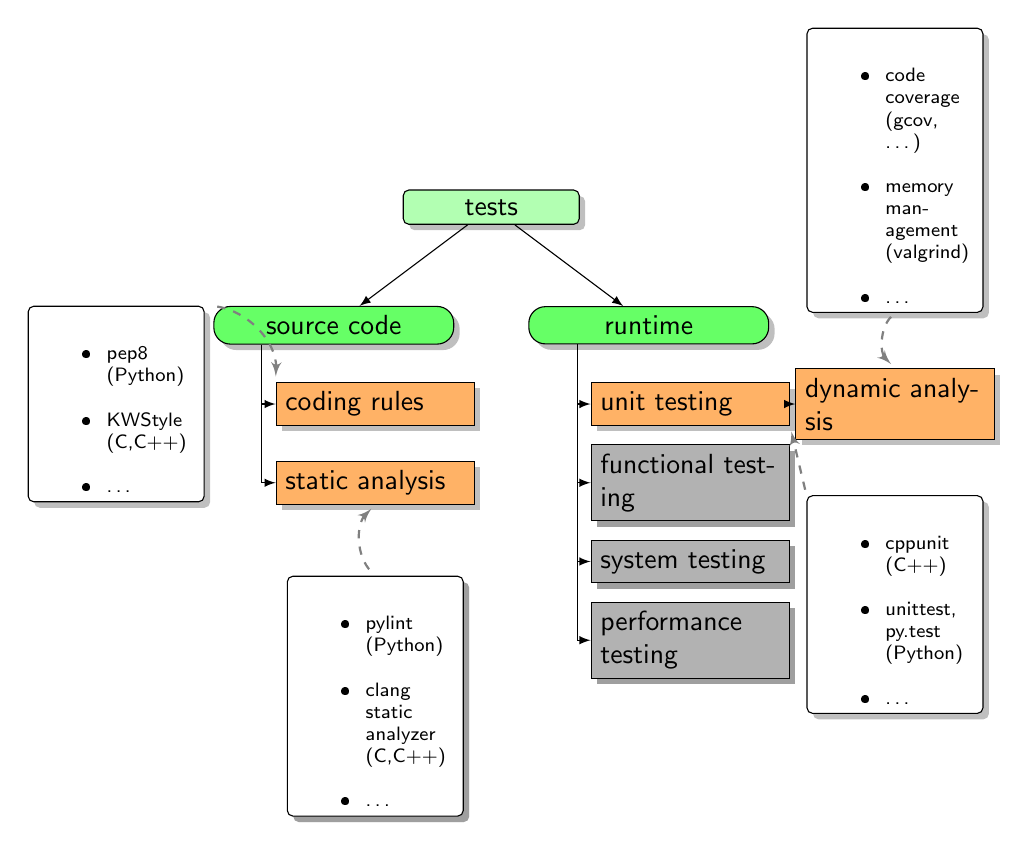
\begin{tikzpicture}[
      level 1/.style={sibling distance=40mm},
      edge from parent/.style={->,draw},
    >=latex]

% root of the the initial tree, level 1
    \node[root] {tests}
% The first level, as children of the initial tree
    child {node[level 2] (c1) {source code}}
    child {node[level 2] (c2) {runtime}};


% The second level, relatively positioned nodes
    \begin{scope}[every node/.style={level 3}]
      \node [below of = c1, xshift=15pt] (c11) {coding rules};
      \node [below of = c11] (c12) {static analysis};
      \node [below of = c2, xshift=15pt] (c21) {unit testing};
      \node [below of = c21,mstep4] (c22) {functional testing};
      \node [below of = c22,mstep4] (c23) {system testing};
      \node [below of = c23,mstep4] (c24) {performance testing};
      \node [right of = c21,xshift=1.6cm] (dynamic_analysis) {dynamic analysis};
      \node [below=.9cm of c12,mstep2b] (static_an) {\scriptsize
\begin{itemize}
        \item pylint (Python)
        \item clang static analyzer (C,C++)
        \item \dots
\end{itemize}

      };
    \end{scope}
      \node[left=.9cm of c11,mstep2b] (codage) {\scriptsize
\begin{itemize}
        \item pep8 (Python)
        \item KWStyle (C,C++)
        \item \dots
\end{itemize}
      };
      \node[above=.7cm of dynamic_analysis,mstep2b] (dynamic_analysis_tools) {\scriptsize
\begin{itemize}
        \item code coverage (gcov, \dots)
        \item memory management (valgrind)
        \item \dots
\end{itemize}

      };
      \node[below=.7cm of dynamic_analysis,mstep2b] (unit_tests_tools) {\scriptsize
\begin{itemize}
        \item cppunit (C++)
        \item unittest, py.test (Python)
        \item \dots
\end{itemize}

      };
      \draw[<-, >=latex', shorten >=2pt, shorten <=2pt, thick, color=gray, bend right=45,dashed]
      (c11.north west) to node[auto, swap] {} (codage.north east);
      \draw[<-, >=latex', shorten >=2pt, shorten <=2pt, thick, color=gray, bend right=45,dashed]
      (c12.south) to node[auto, swap] {} (static_an.north);
      \draw[->, >=latex', shorten >=2pt, shorten <=2pt, thick, color=gray, bend right=45,dashed]
      (dynamic_analysis_tools.south) to node[auto, swap] {} (dynamic_analysis.north);
      \draw[->, >=latex', shorten >=2pt, shorten <=2pt, thick, color=gray,dashed]
      (unit_tests_tools.north west) to node[auto, swap] {} (c21.south east);

% lines from each level 1 node to every one of its "children"
    \draw[->] (c21.east) |- (dynamic_analysis.west);

    \foreach \value in {1,2}
    \draw[->] (c1.195) |- (c1\value.west);

    \foreach \value in {1,...,4}
    \draw[->] (c2.195) |- (c2\value.west);


    % \node [draw,rectangle,fill=gray] at (8,0) {Intégration continue}
    % child {node [draw,rectangle,fill=gray] {compilations automatiques}}
    % child {node [draw,rectangle,fill=gray] {tests automatiques}}
    % child {node [draw,rectangle,fill=gray] {``commits'' journaliers}}
    % child {node [draw,rectangle,fill=gray] {tous les ``commits'' doivent être compilés et testés}}
    % child {node [draw,rectangle,fill=gray] {la compilation doit rester rapide}}
    % child {node [draw,rectangle,fill=gray] {le test ne doit pas se faire dans l'environnement de production}}
    % child {node [draw,rectangle,fill=gray] {les résultats des dernières compilations et tests doivent être visibles}}
    % child {node [draw,rectangle,fill=gray] {le déploiement doit être automatisé}};


   % \node[draw,rectangle,color=black] {Intégration continue}
   % node[] {dépôt du code source \textbf{versionné}}
   % child { node[] {compilations automatiques} }
   % child { node[] {tests automatiques} }
   % child { node[] {``commits'' journaliers} }
   % child { node[] {tous les ``commits'' doivent être compilés} }
   % child { node[] {la compilation doit rester rapide} }
   %    child { node[] {le test ne doit pas se faire dans l'environnement de production} }
   %    child { node[] {le dernier délivrable doit être disponible facilement} }
   %    child { node[] {les résultats des dernières compilations et tests doivent être visibles} }
   %    child { node[] {le déploiement doit être automatisé} }
   %  } ;
  \end{tikzpicture}

\end{frame}

%% \begin{frame}{Which tests ?}

%% %%%% Eclater le slide precedent en 4 slides pour expliquer tests + interest
%% Runtime :
%% - Unit test, functional tests
%% TDD concepts

%% Source code :
%% - Coding rules : why 
%% - Static analysis

%% Quand faire test (centralise et de maniere continu !!!)
%% d'ou faire integration continue
%% \end{frame}


\section{What is continuous integration ?}

\subsection{Principles}

\begin{frame}{}
\begin{block}{Software integration process = build workflow}
\begin{tikzpicture}
  \node[] (developer1) {\includegraphics[width=.04\textwidth] {images/Laptop-icon.png}};
  \node[below=.001cm of developer1] (developer2) {\includegraphics[width=.04\textwidth] {images/Laptop-icon.png}};
  \node[below=.001cm of developer2] (developer3) {\includegraphics[width=.04\textwidth] {images/Laptop-icon.png}};
  \node[right=1.3cm of developer2] (code_repo_db) {};
  \node[above=.4cm of code_repo_db] (code_repo_db_north) {};
  \node[left=.2cm of code_repo_db] (code_repo_db_west) {};
  \node[below=.1cm of code_repo_db] (code_repo_db_south) {};
  \node[below=.9cm of code_repo_db,mstep1] (code_repo) {Source control management};
  \aboxl[25,20,1.6,a1,(code_repo_db)] {};
  \node[right=.6cm of code_repo,mstep2] (build) {Build (static tests)};
  \node[above=.4cm of build] (nux) {\includegraphics[width=.04\textwidth] {images/Linux-icon.png}};
  \node[above=.001cm of nux] (windows) {\includegraphics[width=.04\textwidth] {images/Windows-icon.png}};
  \node[above=.001cm of windows] (freebsd) {\includegraphics[width=.04\textwidth] {images/Apps-freebsd-icon.png}};
  \node[right=.6cm of build,mstep2] (tests) {Tests};
  \node[above=.4cm of tests] (test_ok1) {\includegraphics[width=.02\textwidth] {images/accept-icon.png}};
  \node[above=.001cm of test_ok1] (test_ok2) {\includegraphics[width=.02\textwidth] {images/accept-icon.png}};
  \node[above=.001cm of test_ok2] (test_bad1) {\includegraphics[width=.02\textwidth] {images/delete-icon.png}};
  \node[above=.001cm of test_bad1] (test_ok4) {\includegraphics[width=.02\textwidth] {images/accept-icon.png}};
  \node[right=.001cm of test_ok1] (test_bad1) {\includegraphics[width=.02\textwidth] {images/delete-icon.png}};
  \node[right=.001cm of test_ok2] (test_ok3) {\includegraphics[width=.02\textwidth] {images/accept-icon.png}};
  \node[right=.6cm of tests,mstep2] (install) {Package installation};
  \node[above=.4cm of install] (package) {\includegraphics[width=.06\textwidth] {images/System-Package-icon.png}};
  \path[<->, thick, color=blue] (developer1) edge [bend left] (code_repo_db_north);
  \path[<->, thick, color=blue] (developer2) edge [] (code_repo_db_west);
  \path[<->, thick, color=blue] (developer3) edge [bend right] (code_repo_db_south);
  \path[->, thick, color=gray,dotted] (code_repo.east) edge [] (build.west);
  \path[->, thick, color=gray,dotted] (build) edge [] (tests);
  \path[->, thick, color=gray,dotted] (tests) edge [] (install);
\end{tikzpicture}
\end{block}
\begin{block}{Continuous process}
\begin{itemize}
\item When a new contribution : launch the build workflow
\item And/or regularly : nigthly or weekly integration
\end{itemize}
\end{block}
\end{frame}

\subsection{Purposes}

\begin{frame}{Continuous integration}

  \begin{block}{Why ?}
    A short development cycle to find problems early and avoid pitfalls of ``integration hell''
    \begin{itemize}
    \item Regression tests
    \item Portability regression handling
    \item Merge code handling
    \item \dots
  \end{itemize}

  \textbf{Continuous integration is related to a specific software workflow}

\end{block}

\begin{block}{Implication}
\begin{itemize}
\item Each step of the software workflow needs to be \textbf{automated} : build, tests, package
\item Each step must be launched by an engine
\item A dashboard for results must be available
\end{itemize}
\end{block}
\end{frame}

\subsection{Issues to take into account with automation}
\begin{frame}{Build automation}
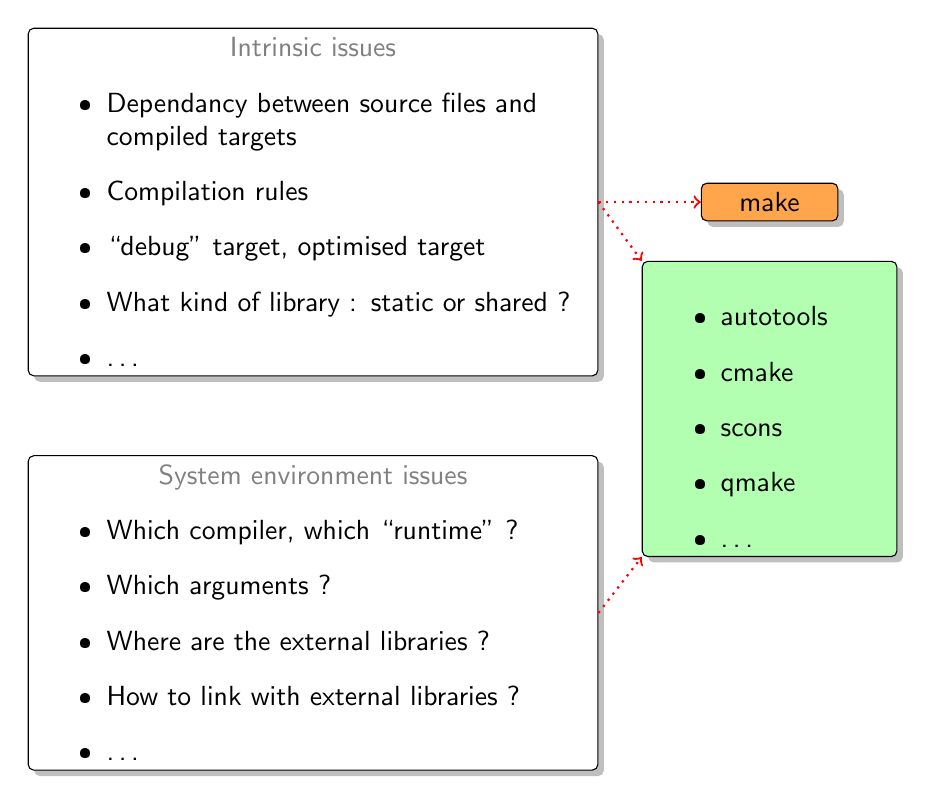
\begin{tikzpicture}
\node[mstep3b] (intrinsics) {
\textcolor{gray}{Intrinsic issues}
  \begin{itemize}
  \item Dependancy between source files and compiled targets
  \item Compilation rules
  \item ``debug'' target, optimised target
  \item What kind of library : static or shared ?
  \item \dots
  \end{itemize}};
\node[below=1cm of intrinsics,mstep3b] (extrinsics) {
\textcolor{gray}{System environment issues}
  \begin{itemize}
  \item Which compiler, which ``runtime'' ?
  \item Which arguments ?
  \item Where are the external libraries ?
  \item How to link with external libraries ?
  \item \dots
  \end{itemize}};
\node [right=1.3cm of intrinsics,mstep1] (make) {make};
\node [below=.5cm of make,mstep3] (build_tools) {
  \begin{itemize}
  \item autotools
  \item cmake
  \item scons
  \item qmake
  \item \dots
  \end{itemize}};

\node[above=.1cm of build_tools] (build_tools_north) {};
\node[below=.1cm of build_tools] (build_tools_south) {};
\path[->, thick, color=red,dotted] (intrinsics.east) edge [] (make.west);
\path[->, thick, color=red,dotted] (intrinsics.east) edge [] (build_tools.north west);
\path[->, thick, color=red,dotted] (extrinsics.east) edge [] (build_tools.south west);
\end{tikzpicture}
\end{frame}

\
\begin{frame}{Typical workflow}
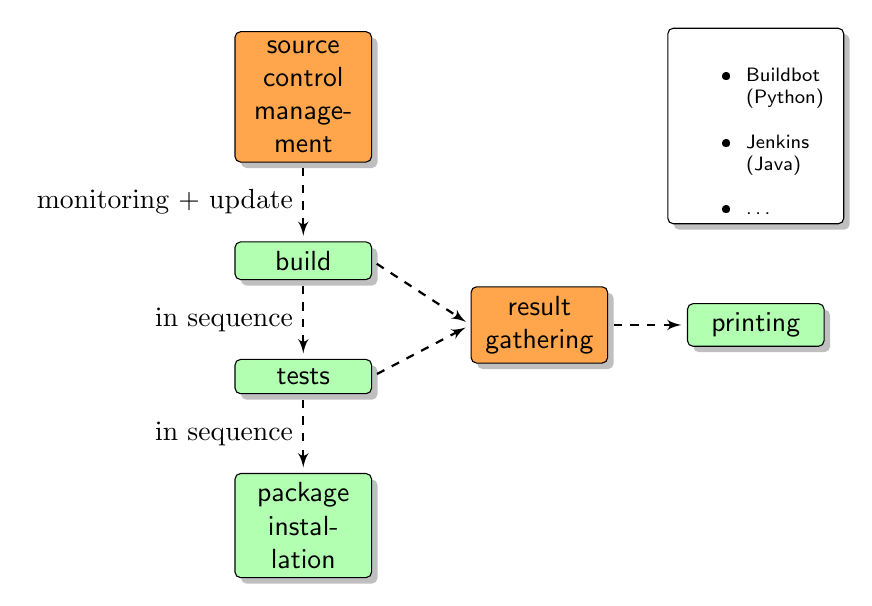
\begin{tikzpicture}
%  \node[mstep1] (integ) { Intégration continue };
  \node[mstep1] (code_repo) {source control management};
  \node[below=1cm of code_repo,mstep2] (build) {build};
  \node[below=1cm of build,mstep2] (tests) {tests};
  \node[below=1cm of tests,mstep2] (install) {package installation};
  \node[right=2cm of build] (build_r1) {};
  \node[below=.2cm of build_r1,mstep1] (build_r) {result gathering};
  \node[right=1cm of build_r,mstep2] (build_r_a) {printing};
  \node[above=1cm of build_r_a,mstep2b] (tools) {\scriptsize 
\begin{itemize}
\item Buildbot (Python) \\
\item \alert{Jenkins} (Java) \\
\item \dots
\end{itemize}
};
  \draw[->, >=latex', shorten >=2pt, shorten <=2pt, thick, dashed]
  (code_repo.south) to node[auto, swap] {monitoring + update} (build.north);
  \draw[->, >=latex', shorten >=2pt, shorten <=2pt, thick, dashed]
  (build.south) to node[auto, swap] {in sequence} (tests.north);
  \draw[->, >=latex', shorten >=2pt, shorten <=2pt, thick, dashed]
  (tests.south) to node[auto, swap] {in sequence} (install.north);
  \draw[->, >=latex', shorten >=2pt, shorten <=2pt, thick, dashed]
  (build.east) to node[auto, swap] {} (build_r.west);
  \draw[->, >=latex', shorten >=2pt, shorten <=2pt, thick, dashed]
  (tests.east) to node[auto, swap] {} (build_r.west);
  \draw[->, >=latex', shorten >=2pt, shorten <=2pt, thick, dashed]
  (build_r.east) to node[auto, swap] {} (build_r_a.west);
%  \path[->,thick,color=gray] (code_repo) edge [] (build);
\end{tikzpicture}
\end{frame}



% L'intégration continue à Inria
% ******************************
\inriaswitchcolors{blue}
\section{Continuous Integration at Inria}

\subsection{Dedicated site : ci.inria.fr}
\begin{frame}{https://ci.inria.fr/}
  \begin{tikzpicture}
    \node[] (root) {};
    \node[below=3.5cm of root] (root_south) {};
    \node[] (ci_main)  {\includegraphics[width=.9\textwidth] {images/ci-main.png}};
    \node[right=1.1cm of root_south,draw,rectangle,thick,drop shadow,color=gray,rounded corners=2pt] (ci_doc)  {\includegraphics[width=.9\textwidth] {images/ci-doc.png}};
    \node[draw,ellipse,minimum height=.8cm,minimum width=2.5cm,thick,color=red] at (.7,0.9) (ok) {};
    \path[->, thick, color=red] (.6,.2) edge [bend right] (.9,-.2);

    \node[above=3cm of root,mstep1] (frontale) {Front-end website};
    \node[right=2cm of frontale] (t0) {};
    \node[above=.5cm of t0,mstep2] (cloudstack) {CloudStack};
    \node[below=.5cm of t0,mstep2] (jenkins) {Jenkins};
    \path[->, thick, color=blue] (frontale.east) edge [] (cloudstack.west);
    \path[->, thick, color=blue] (frontale.east) edge [] (jenkins.west);
  \end{tikzpicture}
\end{frame}

\subsection{Sign Up interface}
\begin{frame}{Sign up}
  \begin{tikzpicture}
    \node[] (root) {};
    \node[below=3.5cm of root] (root_south) {};
    \node[] (ci_main)  {\includegraphics[width=.9\textwidth] {images/ci-signup.png}};
  \end{tikzpicture}
\end{frame}
\subsection{User page}
\begin{frame}{User page}
  \begin{tikzpicture}
    \node[] (root) {};
    \node[below=3.5cm of root] (root_south) {};
    \node[] (ci_main)  {\includegraphics[width=.9\textwidth] {images/ci-user.png}};
  \end{tikzpicture}
\end{frame}

\subsection{Example of  a project using virtual machines}
\begin{frame}{A project}
  \begin{tikzpicture}
    \node[] (project)  {\includegraphics[width=1.2\textwidth] {images/ci-project.png}};
  \end{tikzpicture}
\end{frame}

\begin{frame}{High level interface for the related virtual machines}

\begin{tikzpicture}
 \node[] (project)  {\includegraphics[width=.9\textwidth] {images/ci-slaves.png}};
\end{tikzpicture}
\end{frame}

\begin{frame}{How to create a new virtual machine}
  \begin{tikzpicture}
    \node[] (project)  {\includegraphics[width=.9\textwidth] {images/new-slave.png}};
  \end{tikzpicture}
\end{frame}


\begin{frame}{Access to the virtual machine server : cloudstack}
  \begin{tikzpicture}
    \node[] (project)  {\includegraphics[width=1.2\textwidth] {images/cloudstack-main.png}};
  \end{tikzpicture}
\end{frame}

\begin{frame}{Access to the virtual machine server : cloudstack/machine}
\begin{tikzpicture}
 \node[] (windows_conf)  {\includegraphics[width=1.2\textwidth] {images/cloudstack-windows-conf.png}};
 \node[draw,ellipse,minimum height=.8cm,minimum width=.8cm,thick,color=red] at (2.3,1.6) (select) {};
 \node[draw,rectangle,thick,color=red,rounded corners=2pt] at (-4,-0.4) (windows_desktop) {\includegraphics[width=.4\textwidth] {images/cloudstack-windows-desktop.png}};
 \path[->, thick, color=red] (select.south) edge [bend left] (windows_desktop.east);
\end{tikzpicture}
\end{frame}



\section{Lab assignments}

\subsection{Purpose}


\begin{frame}{Purpose} % {\subsecname}
\begin{itemize}
\item Project with given code + test : to be found in ...
\item Choose Python, C++ or Java code project version
\item Purpose :
\begin{itemize}
\item Add tests in project
\item Configure Jenkins for build
\item Launch Build
\item Launch Chuck Norris
\item Launch Junit
\item Launch Covertura
\end{itemize}
\end{itemize}
\end{frame}

\subsection{Example of Python test}
\begin{frame}[fragile]{\subsecname} % {\subsecname}
\begin{verbatim}
import unittest

class WidgetTestCase(unittest.TestCase):
    def setUp(self):
        self.widget = Widget('The widget')

    def tearDown(self):
        self.widget.dispose()
        self.widget = None

    def test_default_size(self):
        self.assertEqual(self.widget.size(), (50,50),
                         'incorrect default size')

    def test_resize(self):
        self.widget.resize(100,150)
        self.assertEqual(self.widget.size(), (100,150),
                         'wrong size after resize')

\end{verbatim}
\end{frame}

\subsection{Lab assignment steps}
\begin{frame}{\subsecname} % {\subsecname}

\begin{block}{Create user account and join project}
\begin{enumerate}
\item Create an account : Sign Up
\item Log in : beware use email address as login
\item Join project \texttt{XXXX}
\end{enumerate}
\end{block}

\begin{block}{Create a build workflow for project \texttt{XXXX}}
\begin{enumerate}
\item Access Jenkins interface for project \texttt{XXXX}
\item Create a job which name is \texttt{YOURNAME\_[C|JAVA|PYTHON]\_YYY}
\item Create ``Freestyle'' project
\item Configure Build shell tab
\end{enumerate}
\end{block}
\end{frame}

\begin{frame}{Build configuration example}{Jenkins}
  \includegraphics[width=\linewidth]{images/build_configuration}
\end{frame}

\subsubsection{Tools to be used...}
\begin{frame}{Tools setup}

  Gestionnaire de versions: \texttt{git} \\ ~ \\

  \begin{tabular}{ l | l l | p{3.5cm} }
    Language         & \texttt{Python}     & \texttt{C}    & Utiisation dans Jenkins \\ \hline
    Script de build  & \texttt{setuptools} & \texttt{Make} & Bash~shell, \texttt{EnvInject} \texttt{virtualenv}\\
    Compilation      & ~                   & \texttt{gcc}  & ~ \\
    Tests            & \texttt{nose}, \texttt{unittest}, \texttt{mock}
                     & \texttt{gtest} \texttt{(C++)}
                     & Junit, Chuck Norris\\
    Couverture       & \texttt{nose-xcover}
                     & \texttt{gcov}, \texttt{gcovr}
                     & Cobertura \\
   Qualité de code  & \texttt{pylint}, \texttt{pep8} & ~  & Violations \\
                   ~ & ~  & ~ & \\
    Lignes de code   &  $3000$        &  $1500$  &  $0$  \\
    Lignes de tests  &  $1600 + 400$  &  $1300$  &  $0$  \\
% 1600 tests U + 400 tests intégration
    Lignes de build  &  $300$         &  $170$   &  $50$ \\

    \note[item]{Gestion de version, partagée avec d'autres projets}
    \note[item]{Correspondance entre outils mis en place et Jenkins, \textbf{fichiers générés}}
    \note[item]{Types d'outils les uns après les autres}
    \note[item]{Pylint remplace compilation Python}
    \note[item]{}
    \note[item]{1600 tests U + 400 tests intégration}
    \note[item]{SQLite 3.8 == 1084 * plus de tests que de code 84k source (hors blank et commentaires)}
  \end{tabular}
\end{frame}




\begin{frame}{Cobertura}{Jenkins}
        % Pour moi, l'outil le plus important (après Chuck Norris forcément)
  \includegraphics[width=\linewidth]{images/cobertura}\\
\end{frame}
\begin{frame}{Junit - Violations}{Jenkins}
  \begin{center}
        % Juste pour montrer
    \includegraphics[height=0.8\textheight]{images/junit_violations}\\
  \end{center}
\end{frame}
\begin{frame}{Chuck Norris}{Jenkins}
  % Le plus important des plugins
  \begin{center}
    \begin{tabular}{ l |l }
      Build KO & Build OK \\ \hline
        \includegraphics[height=4cm]{images/chuck_full} &
      \includegraphics[height=4cm]{images/chuck_happy}
        %\includegraphics[height=4cm]{images/chuck_angry}
      \\
    \end{tabular}
  \end{center}
  Chuck Norris Facts:
  \begin{itemize}
    \item Chuck Norris can unit test an entire application with a single assert.
    \item Chuck Norris can divide by zero.
    \item ...
  \end{itemize}
\end{frame}



\begin{frame}{The End}
  Questions ?  Remarks ?
\end{frame}


\end{document}
